\documentclass[a4paper,ngerman,landscape]{scrartcl}

\usepackage[utf8]{inputenc}

\usepackage[ngerman]{babel}
\usepackage{hyperref}

\usepackage{graphicx}

\usepackage[protrusion=true,expansion=true]{microtype}

\usepackage{libertine}
\usepackage{tabto}

\setlength\parskip{\medskipamount}
\setlength\parindent{0pt}

\usepackage{geometry}
\geometry{tmargin=0.1cm,bmargin=1.0cm,lmargin=2.5cm,rmargin=2.5cm}

\pagestyle{empty}

\begin{document}

\begin{center}
  \Huge
  \vspace*{0.0em}
  Freitag, 21. Oktober 2016, 14:00 Uhr, 1005/L1 \\
  \mbox{\textbf{Ingo Blechschmidt: Das Geheimnis der Zahl 5}}
  \vfill
  % https://en.wikipedia.org/wiki/File:Sunflowers.jpg
  \vspace{0.3em}
  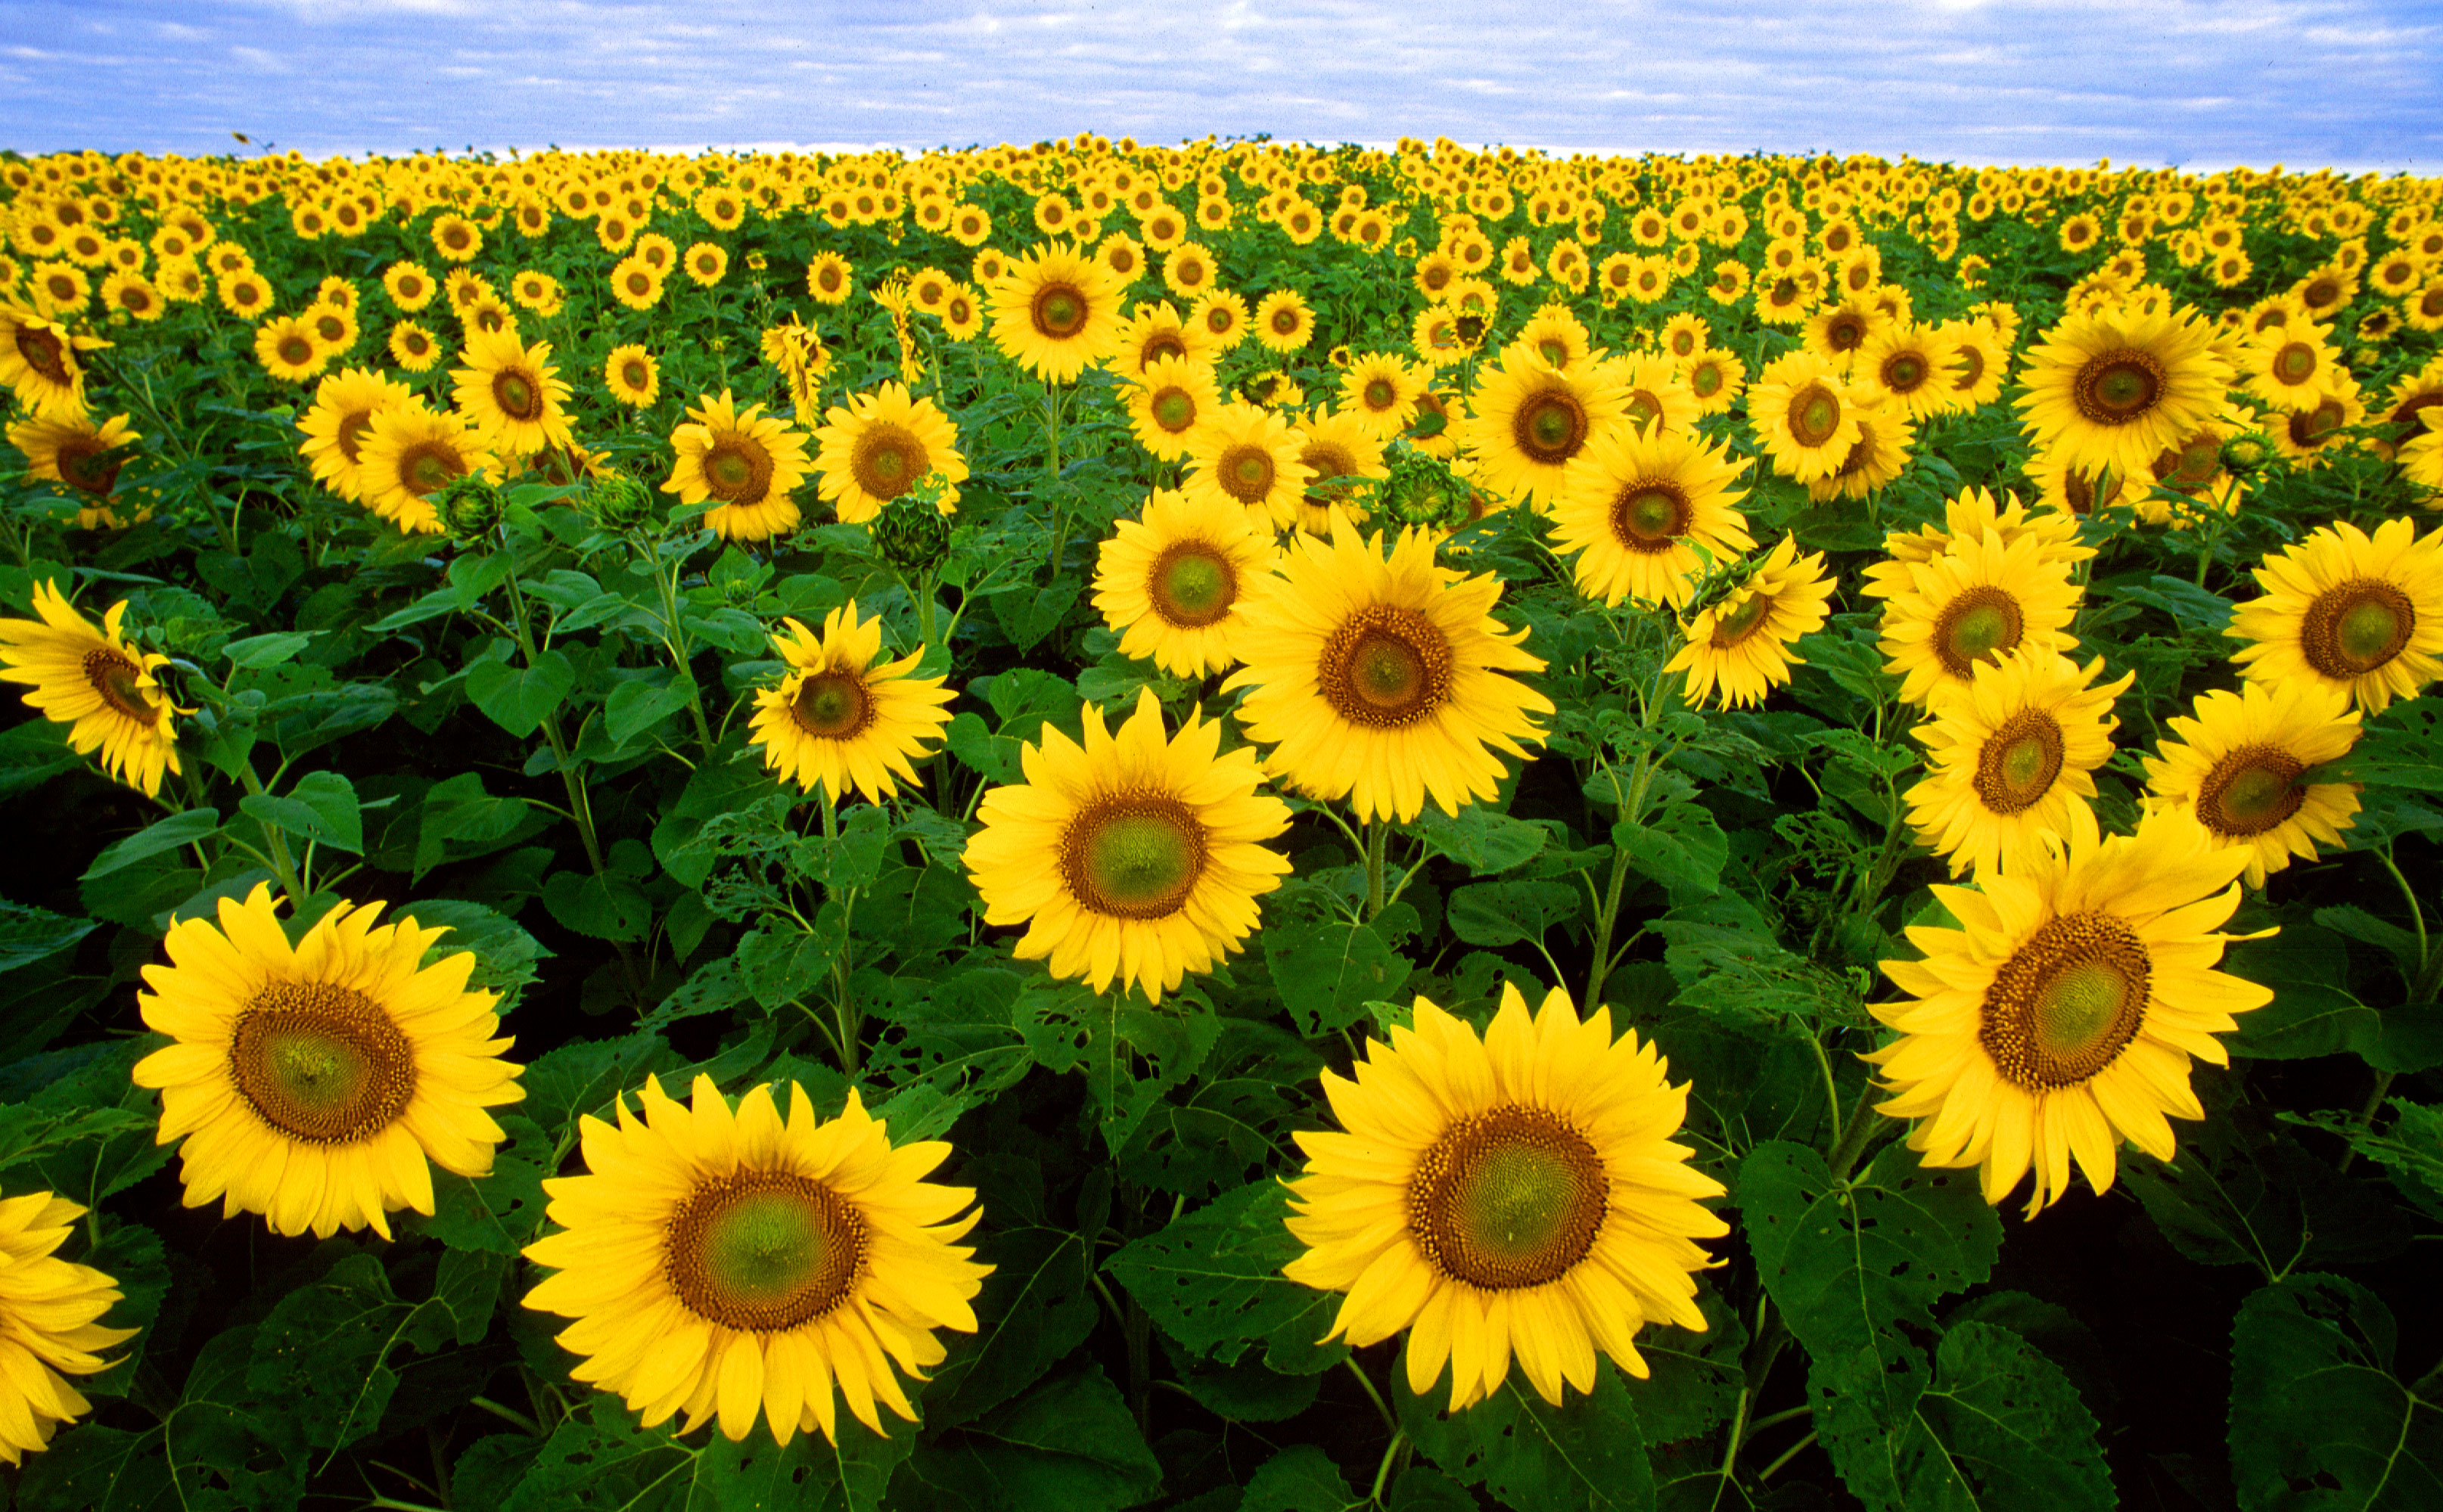
\includegraphics[width=0.6\textwidth]{sonnenblumen}
  \vfill

  \Large
  \begin{minipage}{0.92\textwidth}
    \setlength\parskip{\medskipamount}
    \vspace{0.3em}
    Was ist der goldene Schnitt? Wieso kommt er nicht nur in der Kunst, sondern
    auch in der Natur überall vor? Was hat der goldene Schnitt mit den
    Fibonacci-Zahlen zu tun (1, 1, 2, 3, 5, 8, 13, \ldots)? Wieso kann die Ananas
    aus Spongebob Schwammkopf keine echte Ananas sein? Wie könnten die
    Mathematikerinnen und Mathematiker der Antike auf die erstaunlich guten
    Näherungen $22/7$ und $355/113$ der Kreiszahl Pi gekommen sein? Welch
    glücklicher Zufall der Mathematik spielte dabei eine Rolle? Was ist der
    tiefere Grund dafür, dass der Schokoladentrick ("`ein Kästchen
    verschwindet"') funktioniert? Und was hat das alles mit der Zahl 5,
    unendlich verschachtelten Brüchen und dem Apfelmännchen-Fraktal zu tun?

    Der Vortrag setzt nur Schulkenntnisse voraus. Alle Interessierten sind
    herzlich eingeladen. Vielleicht gibt es Kekse. Der Vortrag ist Jost-Hinrich
    Eschenburg gewidmet.
    \vspace{0.3em}
    \hfill\small Skript und Übungsblätter: \textsf{http:/$\!$/pizzaseminar.speicherleck.de/}
  \end{minipage}
\end{center}

\begin{center}
  \vspace*{1.5em}
  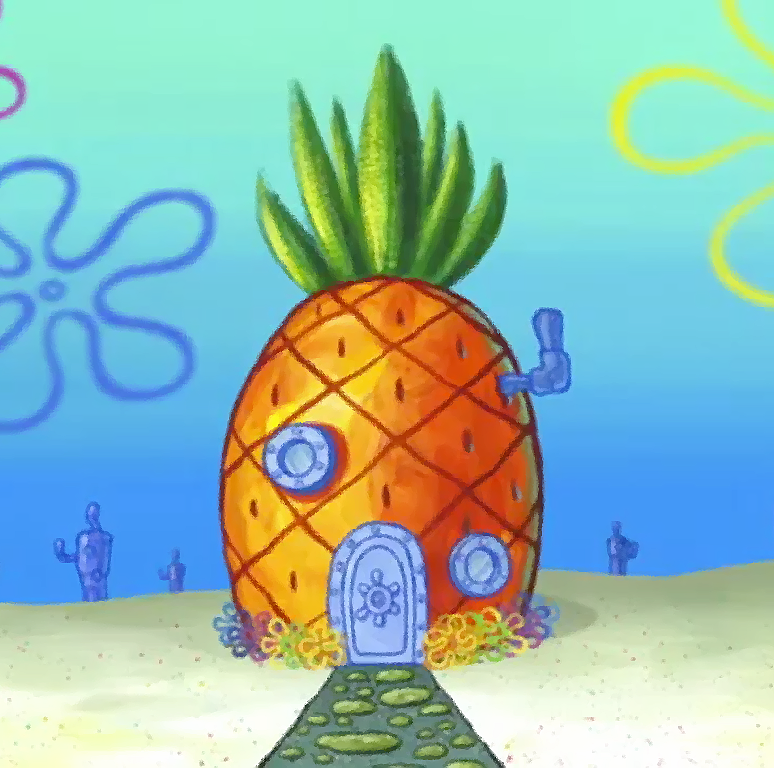
\includegraphics[height=0.9\textheight]{spongebob-ananas}
  \begin{minipage}[b]{0.25\textwidth}
  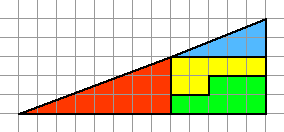
\includegraphics[width=\textwidth]{ein-kaestchen-verschwindet-1}
  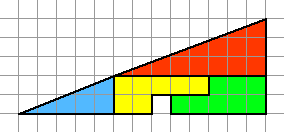
\includegraphics[width=\textwidth]{ein-kaestchen-verschwindet-2}

  \bigskip
  \bigskip
  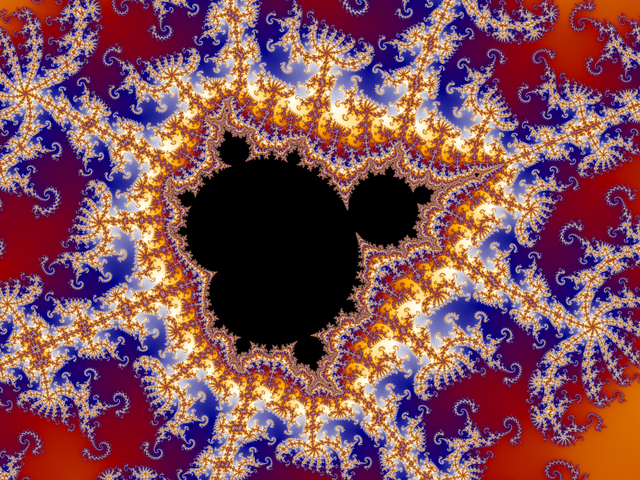
\includegraphics[height=0.32\textheight,angle=90]{mandelbrot}
  \end{minipage}
  \vfill
  \newpage
  \vspace*{1.5em}
  \Huge
  \scalebox{2.3}{Geh da nicht hin!} \\[0.8em]
  \scalebox{2.3}{\textbf{Verbotener Geheimvortrag.}} \\[0.8em]
  \vspace{0.2em}

  Freitag, 21. Oktober 2016, 14:00 Uhr, 1005/L1 \\
  \mbox{\textbf{Ingo Blechschmidt: Das Geheimnis der Zahl 5}}
  \vspace{1em}

  \huge
  \begin{minipage}{0.99\textwidth}
    \setlength\parskip{\medskipamount}
    Was ist der goldene Schnitt? Wieso kommt er nicht nur in der Kunst, sondern
    auch in der Natur überall vor? Was hat der goldene Schnitt mit den
    Fibonacci-Zahlen zu tun (1, 1, 2, 3, 5, 8, 13, \ldots)? Wieso kann die Ananas
    aus Spongebob Schwammkopf keine echte Ananas sein? Wie könnten die
    Mathematikerinnen und Mathematiker der Antike auf die erstaunlich guten
    Näherungen 22/7 und 355/113 der Kreiszahl Pi gekommen sein? Welch
    glücklicher Zufall der Mathematik spielte dabei eine Rolle? Was ist der
    tiefere Grund dafür, dass der Schokoladentrick ("`ein Kästchen
    verschwindet"') funktioniert? Und was hat das alles mit der Zahl 5,
    unendlich verschachtelten Brüchen und dem Apfelmännchen-Fraktal zu tun?

    Der Vortrag setzt nur Schulkenntnisse voraus. Alle Interessierten sind
    herzlich eingeladen. Vielleicht gibt es Kekse. Der Vortrag ist Jost-Hinrich
    Eschenburg gewidmet.
    \vspace{0.3em}
  \end{minipage}
\end{center}

\end{document}
